\section{Optimale Parameter}

Die folgenden Parameter sind laut unseren Messungen ideal: \\

\begin{tabular}{l c l}
  NumberIndividuals   & = & 100       \\
  NumberSubpopulation & = & 5         \\
  Migration.Interval  & = & 1         \\
  Migration.Rate      & = & 0.25      \\
  Migration.Topology  & = & 1 (nur zw. nächsten Nachbarn) \\
  Migration.Selection & = & 1 (nur beste Individuen)      \\
  Selection.Name      & = & seltour   \\
  Recombination.Name  & = & recox     \\
  Mutation.Name       & = & mutmove   \\
  Mutation.Rate       & = & 1.25 \\\\
\end{tabular}

\noindent Wenn das Skript mit diesen von uns als ideal betrachteten
Parametern inizialisiert wird, erhalten wir in einigen Iterationen
das \emph{ideale Ergebnis von 2020 Kilometern} der Rundreisestrecke.
Siehe dazu Tabelle \ref{tspOpt} und das zugehörige Diagramm
auf Abbildung \ref{fig.tspOpt}.
Auf Abbildung \ref{fig.optPath} ist zudem die Visualisierung des
Reiseweges durch die 29 größten bayrischen Städte zu sehen.
\emph{Anmerkung:} Dieser beste Weg kann in verschiedenen Permutationen kodiert sein,
unsere Simulation hat u.a. diese Permutation gefunden:

\noindent $3 \rightarrow 29 \rightarrow 26  \rightarrow 5 \rightarrow  9 \rightarrow 12 \rightarrow  6 \rightarrow 28 \rightarrow  1 \rightarrow 21 \rightarrow 13 \rightarrow 16 \rightarrow 24 \rightarrow  8 \rightarrow 27 \rightarrow 23 \rightarrow  7 \rightarrow 25 \rightarrow 19 \rightarrow 11 \rightarrow 22 \rightarrow 14 \rightarrow 17 \rightarrow 18 \rightarrow 15 \rightarrow  4 \rightarrow 10 \rightarrow 20 \rightarrow  2$

\input{Chapters/gen/tspOpt}

\begin{figure}[h!]
  \centering
  \includegraphics[width=1.0\textwidth]{Figures/gen/tspOpt.png}
  \caption{Ergebnisse mit der endgültigen Konfiguration}\label{fig.tspOpt}
\end{figure}

\begin{figure}[!h] \centering
  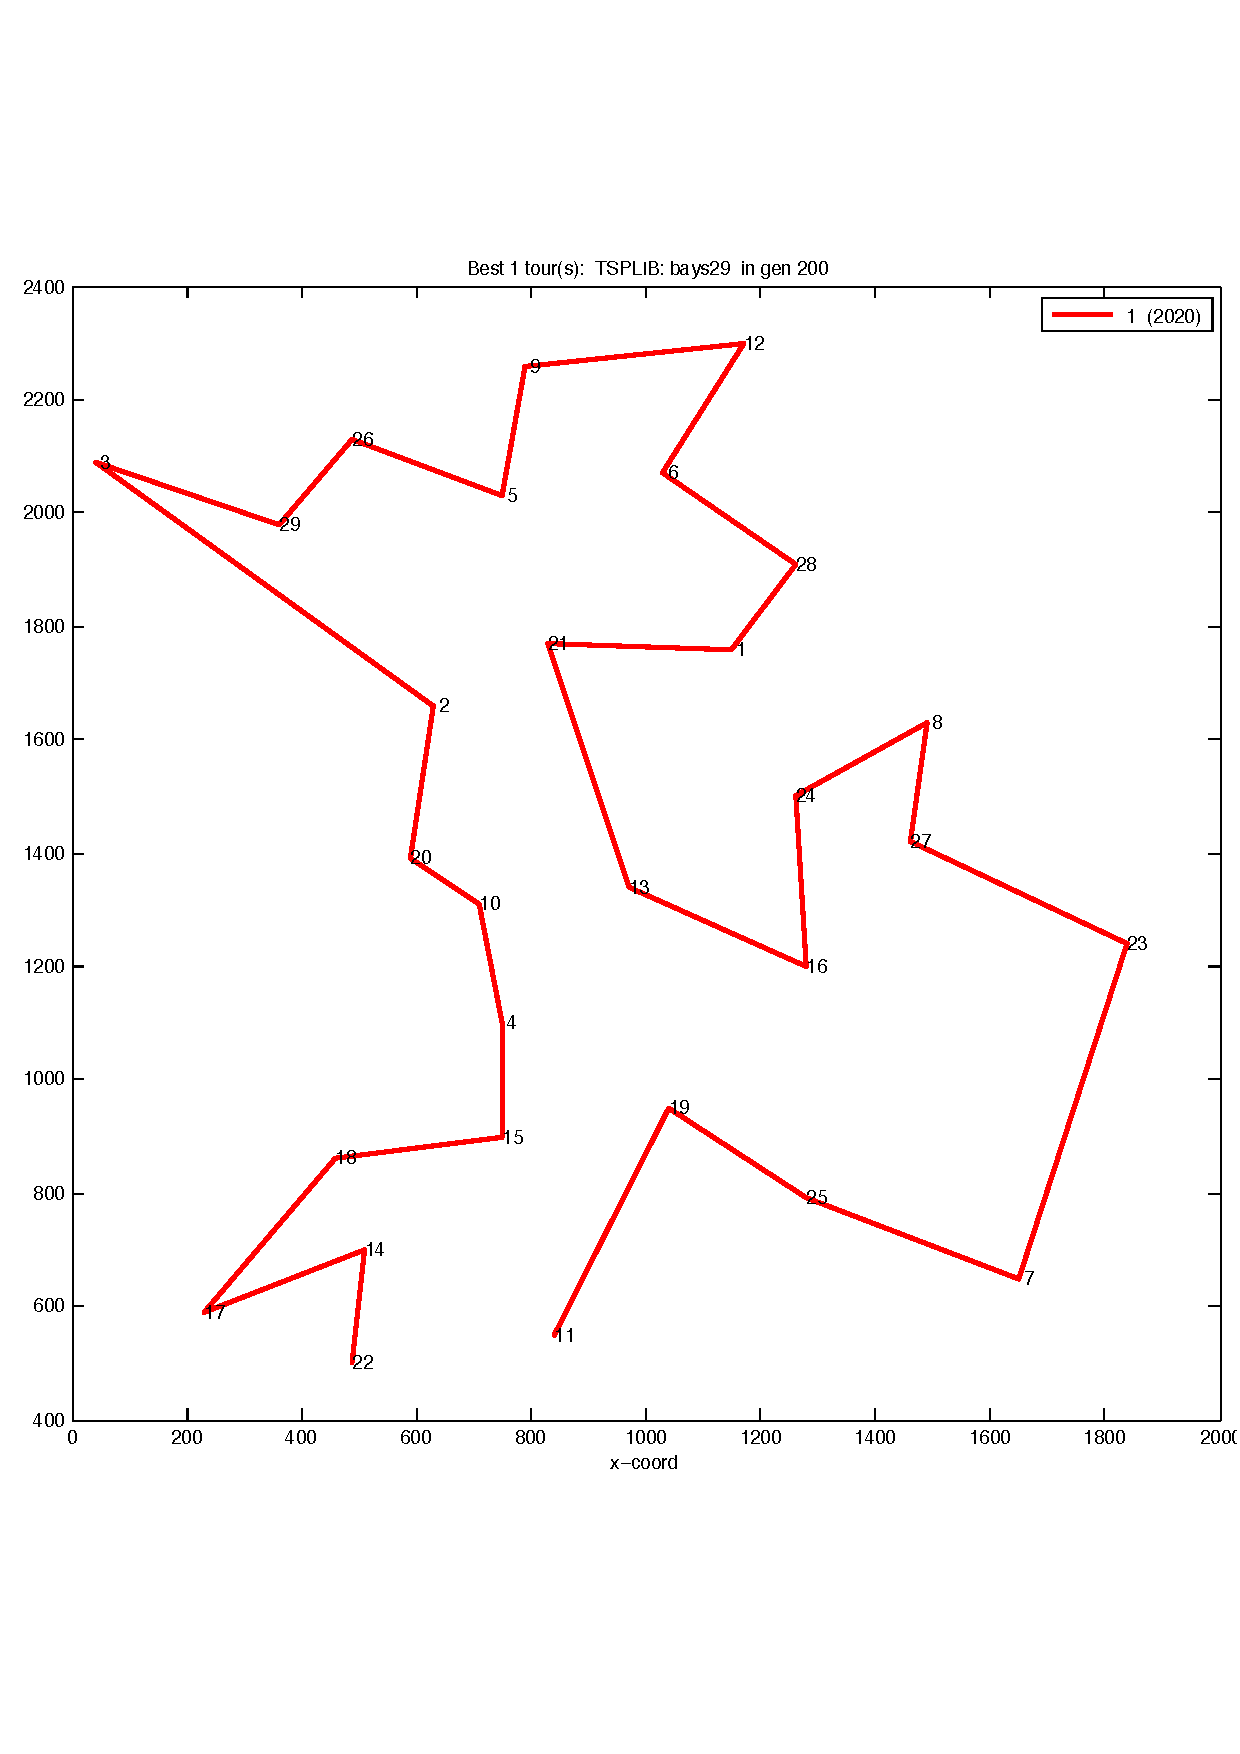
\includegraphics[width=1.0\textwidth]{Figures/path.pdf}
  \caption{Visualisierung des kürzesten Weges (2020km).}
  \label{fig.optPath}
\end{figure}



\section{Fazit}\label{conclusion}

Wir konnten das Travelling Salesman Problem
mit einem evolutionären Algorithmus effizient lösen
und sogar das \emph{optimale} Ergebnis finden, obwohl heuristische
Optimierungsverfahren nicht notwenigerweise die optimalste Lösung finden müssen
(sondern nur annährend optimale Lösungen).

Der Algorithmus liefert mit nicht optimierten Parametern eine Rundreisestrecke
von 2764 km (Mimimum aus 15 Iterationen).
Nach unseren Versuchen konnten wir optimale Parameter ausmachen und mit diesen
das Skript laufen lassen: dort lag das Minimum bei 2020 km, was laut Aufgabenstellung
die optimale Lösung darstellt.
Es sei angemerkt, dass nicht jede Iteration das optimale Ergebnis findet,
jedoch nach insgesamt 25 Iterationen konnten drei Iterationen das optimale
Ergebnis liefern und im Mittelwert lag das Ergebnis bei 2124 km,
also immer sehr nah an der idealen Lösung.

Unser Testsystem war so aufgebaut, dass es die einzelnen Simulationsiterationen
in Textdateien loggt, danach hat ein Pythonskript die Auswertung vorgenommen und
Tabellen sowie Diagramme für dieses LaTeX-Dokument generiert.
Dadurch war viel automatisiert, was den Autoren die Gewissheit gibt, immer die
aktuellsten Simulationsergebnisse konsistent im Dokument zu haben.